\documentclass[12pt]{article}
\usepackage{fancyhdr}
\usepackage{lastpage}
\usepackage{geometry}
\usepackage{amsmath}
\usepackage{setspace}
\usepackage{graphicx}
\usepackage{caption}
\geometry{a4paper,scale=0.8}
\pagestyle{plain}
\renewcommand{\headrulewidth}{0.4pt}
\renewcommand{\footrulewidth}{0.4pt}
\setlength{\baselineskip}{23pt}


\begin{document}
	\thispagestyle{plain}
	\noindent \Large \textbf{The Fama-French Three-Factor Model, Revisited}\\ \\
	\noindent Jin, Kim, Quek, Wang and Woon (2019)\\
	\noindent \normalsize \textit{Singapore Management University, Singapore}\\ \\
	\noindent April 2019, working paper, final version pending
	
		\section{Abstract} % Numbered section
	
		This paper outlines the results of a validity test we have conducted on the Fama and French (1993) three-factor model on eligible stocks listed in NYSE, NASDAQ and AMEX for the period between July 2011 to December 2018. Data on monthly stock returns, monthly 1-month T-bill yields and annual company fundamentals were obtained for the specified period in order to replicate the study. The monthly excess returns suggest that larger-sized companies (i.e. Big-sized) have higher excess returns than portfolios containing smaller sized firms on an average. On the other hand, portfolio constructed of low book-to-market ratio firms look to perform better than those constructed of high book-to-market ratio firms. Quintiles, i.e. twenty-five portfolios, are constructed in accordance to size and book-to-market ratio to help explain the variations on excess portfolio returns by using market risk factor, size risk factor and book-to-market ratio risk factors. After conducting analysis and several statistical tests, we have arrived at the conclusion that Fama and French (1993) three-factor model does display explanatory power over the quintiles given the R-squared and AIC (Akaike information criterion, results shown at Section 6, even though a few quintiles, i.e.  Big-sized with Book-to-Market equity (ranked from 2-4) and Low Book-to-Market equity (ranked at 2) quintiles, proved that the coefficients of the SMB and HML might be statistically insignificant respectively from the derived t-statistics value at 95\% significance level.
	
	
	\section{Introduction \& Literature Review} % Numbered section
	
	The emergence of Modern Portfolio Theory introduced by Markowitz (1952) has set the foundation for portfolio management research, and has spurred an outpouring of research of a similar focus. The Capital Asset Pricing Model (CAPM) developed by harpe (1964), Lintner (1965) and Black (1972) is a result of such an outpouring. The CAPM attempts to explain stock returns using excess market returns as an all-encompassing risk factor, an idea which was quickly popularised, but has since been met with much scrutiny and many empirical contradictions. Amongst the critics of the CAPM are Fama and French (1993), who have built a case arguing that market excess returns alone do not fully explain cross-sectional variations in equity returns and that the addition of two empirically-backed factors are better explaining said variations. The model is also known as the Fama and French (1993) three-factor model:
	
	$$
	R(t) - R_f(t) = a+ b(R_{mkt} - R_f) + s(SMB) + h(HML) +\epsilon_i
	$$
	
	\noindent The three-factor model introduced by Fama and French (1993) has come a long way in shaping views about drivers of stock returns in academia and in practice. On top of the market $\beta$ factor proposed and popularised by Sharpe (1964), Lintner (1965) and Black (1972) in their Capital Asset Pricing Model (CAPM), Fama and French (1993) proposed two additional and empirically-backed factors for the explanation of stock returns: Size (ME) and Book-to-Market Equity (BE/ME). \\
	
	\noindent The three-factor model was proposed in response to several discovered empirical contradictions to the CAPM highlighted in Fama and French (1992a). For one, Banz (1981) found that Size (proxied by Market Equity, or ME) adds explanatory power to cross-sectional average returns provided by market $\beta$s. Also, Bhandari (1988) found a positive relationship between firm leverage and average stock returns. To add, Rosenberg, Reid and Lanstein (1985) and Stattman (1980) discovered a positive relationship between Book-to-Market Equity and average U.S. stock returns. Further, Basu (1983) found that earning-price ratios (E/P) help in the explanation of cross-sectional U.S. stock returns when used in conjunction with size and market $\beta$ factors. These findings contradict the viewpoint that market $\beta$s alone are sufficient in describing cross-sectional expected stock returns. \\
	
	\noindent Amongst the potential and empirically-backed factors for stock returns mentioned earlier, Fama and French (1992a) found that Size (ME) and Book-to-Market (BE/ME), when used together, appear to absorb the roles played by leverage and E/P as explanatory factors for stock returns. it was also discovered that Size and Book-to-Market are able to well-explain cross-sectional average returns for stocks listed on the NYSE, Amex and NASDAQ for the period between 1963 to 1990. This discovery laid the groundwork for the three-factor model proposed by Fama and French (1993).\\
	
	\noindent In their study, Fama and French (1993) divided eligible common stocks traded on the NYSE, Amex or NASDAQ into six portfolios based on their Size and Book-to-Market Equity. Size was proxied by Market Equity (ME), and stocks were determined to be Big (B) or Small (S) based on whether they were above or below the median NYSE ME. Stocks were also determined to have Low (L), Medium (M) or High (H) Book-to-Market Equity based on whether they belonged to the bottom 30\%, middle 40\% or top 30\% of NYSE BE/ME. The resulting six portfolios formed were: S/L, S/M, S/H, B/L, B/M and B/H. Monthly Size (SMB) and Book-to-Market Equity (HML) factor readings were then constructed from the returns of these six portfolios. The Market factor was proxied by $R_M - R_F$, where $R_M$ is the result of the value-weighted return of eligible common stocks and $R_F$ is the one-month U.S. Treasury bill rate. Data relating to the study were obtained from the CRSP and COMPUSTAT.\\
	
	\noindent Fama and French (1993) then proceeded to use the same eligible stocks (used in the SMB and HML factor constructions) to construct 25 portfolios based on their Size and Book-to-Market Equity quintiles. The monthly excess returns of these 25 portfolios were then used as the dependent variables for regressions against the Market, Size and Book-to-Equity factors (the independent variables). It was found that, when used together, the three stock market factors were able to explain most of the variation in the returns of the 25 portfolios.\\
	
	\noindent It was also found that the SMB slope coefficients decreased monotonically as portfolio Size increased, whilst the HML slope coefficients increased monotonically as portfolio Book-to-Market Equity increased. Further, the regression intercepts were found to be mostly statistically indifferent from zero. On the other hand, when the Market factor was the only independent variable in the regressions, lower $R^2$ values were obtained and the Size effect seen in the intercepts discovered by Banz (1981) appeared. Overall, the results of the study offered compelling evidence in support of Size and Book-to-Market Equity as additional explanatory factors for stock returns.\\
	
	\noindent With all that said, the three-factor model is not without its criticisms. For instance, Daniel and Titman (1997) argued that it is the firm characteristics (e.g. region, industry, related lines of business etc), not the covariance structure of returns that actually explain the cross-sectional variation in stock returns. Daniel and Titman (1997) discovered that, once firm
	characteristics were controlled for, expected returns did not seem to be positively related to Market, SMB and HML loadings. The study was conducted for returns over 20.5 years between July 1973 to December 1993. Davis, Fama and French (2000), however, rebutted with their own findings with a higher-powered test, owing to a longer test period of 68 years between July 1929 and June 1997.\\
	
	\noindent Further, a plethora of subsequent studies successfully replicating the insights obtained from Fama and French (1993) for different regions and for different time periods have lent further credence to the notion that the Size and Book-to-Market Equity factors are indeed viable additions to the Market factor as explainers of stock returns.\\
	
	\noindent In recent times, there have been motivations to add more risk factors onto the original Fama and French (1993) three-factor model. Fama and French (2015) extended their original three-factor model by suggesting two additional factors: profitability (Robust Minus Weak, RMW), and investment, (Conservative Minus Aggressive, CMA). There have also been several calls elsewhere to add other risk factors such as momentum and low-volatility as part of the original three-factor model. \\
	
	\noindent Regardless, we are inspired to validate the original Fama and French (1993) three-factor model, albeit in a more modern time, between July 2011 to December 2018. As such, our research null hypothesis is as follows:\\
	
	``\textit{The three stock-market factors suggested by Eugene F. Fama and Kenneth R. French in their 1993 paper titled “Common Risk Factors in the Returns on Stocks and Bonds” do not significantly explain the returns of stocks listed on the NYSE, NASDAQ and AMEX for the period between July 2011 and December 2018.}" \\

	\noindent which if disproved, further validates the findings of Fama and French (1993), even in today's age.
	
\newpage
		
\section{Data, Research Design \& Methodology}
\noindent \textbf{Research Sample}\\
\noindent Our data sample includes data on all eligible stocks listed on the NYSE, NASDAQ and AMEX for the period between July 2011 to December 2018. Monthly data was used to calculate factor realisations and portfolio returns.\\

\noindent \textbf{Data Source: Wharton Research Data Services (WRDS)}\\
Wharton Research Data Services (WRDS) provided us with the following necessary databases Fama and French (1993) utilised in their original study: Center for Research in Security Prices (CRSP), Compustat - Capital IQ and the CRSP/Compustat Merged Database (CCM). \\

\noindent \textbf{Center for Research in Security Prices (CRSP)}\\
\noindent The Center for Research in Security Prices (CRSP) provided us with relevant data on the monthly closing price, returns and outstanding number of eligible stocks. We used PERMCOs and PERMNOs as unique entity and issue identifiers when navigating the CRSP database.\\

\noindent \textbf{Compustat - Capital IQ}\\
\noindent Compustat provided us with relevant data on total stockholders' equity, deferred taxes, investment tax credit and the book value of preferred stock. We used GVKEY as unique entity-level identifiers when navigating the Compustat database.\\

\noindent \textbf{CRSP/Compustat Merged Database (CCM)}\\
\noindent A common misconception is that the CCM database has seamlessly merged CRSP stock market data with Compustat accounting data. We found that this is not the case. The CCM database merely allows for Compustat-included data items to be searched for and linked with CRSP's PERMNO and PERMCO at the issue and entity level respectively, though it was found that GVKEYs and PERMCOs are not exclusive to each other. This means that a GVKEY may correspond to many PERMCOs and vice versa. \\

\noindent Thus, obtaining a complete data link between CRSP and Compustat data required an additional step of creating a new, truly unique entity-level identifier. A new identifier called "GVKEY PERMCO" was created for purposes of traversing between datasets.
For example, if Apple Inc’s GVKEY is 1690 and its PERMCO is 7, its GV KEY PERMCO is 16907, which is a unique identifier. Eventually, the CCM was used only for purposes of matching GVKEYs to PERMCOs, then raw data was obtained from standalone datasets.\\

\noindent \textbf{Factor Construction}\\
$$
R_{i_t}-R_{f_t}=\alpha_{it}+b_{it}(R_{M_t}-R_{f_t})+s_{i_t}(SMB)+h_{i_t}(HML)+\epsilon_{i_t}
$$
\textbf{Rm-Rf}\\
The excess portfolio return in month t, $(R_{M_t}-R_{f_t})$, is the excess market portfolio return in month t. In this study, we construct our own market portfolio to estimate the market return. When making the market portfolio, we add up market equity data of all the eligible stocks, regarding that we are buying all the stocks in the whole market as a portfolio. And we use the market size changes of this portfolio to calculate the return which is exactly market return $R_m$. Additionally 1-month T-bill rates are used as a proxy for the risk free rate.\\ \\
\textbf{BE and ME}\\
We obtained Book Equity (BE) and Market Equity (ME) data from CRSP and Compustat and further more validated it with the data we got from Bloomberg, they matched correspondingly. Then we calculated book-to-market(BE/ME) ratio of each stock and placed all NYSE eligible stocks into three BE/ME group which is high (H), medium (M) and low (L) group based on the breakpoints for the top 30\%, middle 40\% and bottom 30\%. And further more we divided all stocks into five quantile portfolio based on their relative sequence in order to construct our 25 portfolio returns.\\ \\
\textbf{Size}\\
Eligible stocks are allocated to two groups which are small or big (S or B),based on whether their market equity(ME) is below or above the median ME for all NYSE stocks each year. And this time we develop the 5 quantile potrfolios for later usage. \\ \\
\textbf{SMB and HML}\\
\noindent For each month SMB is the difference between the average of the returns on the three small-stock portfolios (S/L, S/M and S/H) and the average of the returns on the three big stock portfolios (B/L, B/M and B/H).
$$
SMB=[(S/L+S/M+S/H)-(B/L+B/M+B/H)]/3
$$
HML is the difference between the average of the returns on the two high-BE/ME portfolios (S/H and B/H) and the average of the returns on the two low-BE/ME portfolios (S/L and B/L).
$$
HML = [(S/H+B/H)–(S/L+B/L)]/2
$$
\noindent \\ \textbf{Regression variable generation: 25 portfolios' return}\\
After the construction of SMB and HML portfolios for independent regression variables, 25 portfolios are constructed with a similar procedure in order to calculate excess portfolio returns for each month. All  stocks used in the analysis are sorted by size and distributed into five groups (s1 to s5) such that each group contains the correspounding quantile portfolio's return respect to SIZE and s1 contains stocks with smallest market cap, s5 with the biggest ones. Moreover, stocks are independently allocated to another five groups (b1 to b5) based on the book-to-market equity (BE/ME). 25 portfolios are constructed as the intersection of the five size groups and five BE/ME groups. For example, s5/b1 portfolio is constructed by the stocks in the biggest fifth of firms and the lowest fifth of BE/ME ratio.\\ 

\noindent \textbf{Issues in/Limitations of the Databases}
\begin{itemize}
	\item Missing Data: E.g. No returns data available when there should be
	\item Incomplete Dataset: CRSP \& Compustat do not cover the whole population of NYSE, NASDAQ and Amex traded stocks, only an overlap of the two datasets is available (only LS, LC and LU CCM-linked data was used)
	\item Repeat Data: Multiple reporting of same company for same period, these companies were excluded out of the sample
	\item Conflicting Data: Standalone CRSP \& Compustat vs. CCM reported different numbers, standalone data readings were deferred to
	\item Computational Cost: Takes hours to compute several million cells due to hardware limitations
\end{itemize}
\section{Summary of Statistics}
\textbf{The explanatory variables}

\noindent The table below gives mean, standard deviation and test statistics for the three explanatory variables. The mean of market risk premium, 0.82\%, which implies 9.84\% on the annual basis, is much higher than what Fama and French reported (0.43\%) for their test period during 1963-1991. Neither SMB nor HML are as significant as market risk premium given their higher p-values. This suggests returns of small caps minus large cap and returns of high BE/ME minus low BE/ME are indifferent from 0.


\begin{figure}[h]
	\centering
	\caption*{Table 1: Stats of Explanatory Variables}
	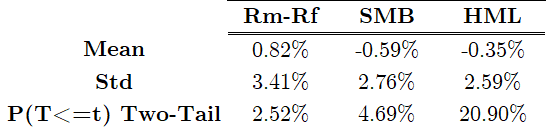
\includegraphics[width=0.5\linewidth]{A1.png}
	\label{fig:label}
\end{figure}


\noindent The correlation matrix shows HML has little correlation with market risk premium and SMB. This implies HML brings in additional explanatory power that CAPM is not able to capture.

\begin{figure}[h]
	\centering
	\caption*{Table 2: Correlation among Explanatory Variables}
	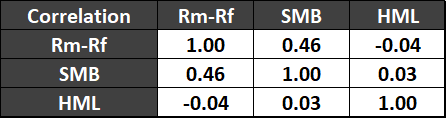
\includegraphics[width=0.35\linewidth]{A2.png}
	\label{fig:label}
\end{figure}


\subsection{The dependent variables}   

Table below lists average of annual number of firms in each portfolio. 61.7\% of firms lie in the union of smallest cap quintile and lowest BE/ME quintiles (as highlighted).



\begin{figure}[h]
	\centering
	\caption*{Table 3: Number of Firms}
	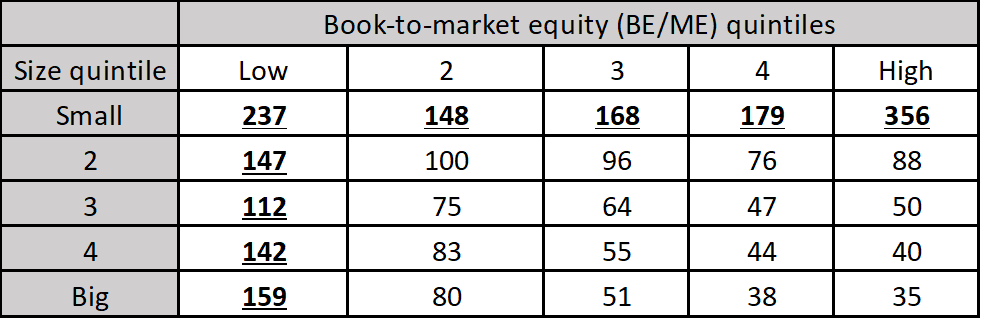
\includegraphics[width=0.5\linewidth]{A3.png}
	\label{fig:label}
\end{figure}

\noindent The table below demonstrates average of monthly excess return for all 25 portfolios between 2011-2018. We are able to find a clear trend that excess returns get higher when size increase in each BE/ME quintiles. On the other hand, we can see lower BE/ME portfolios yields higher excess return in size quintiles “3” and “Big”, but the consistency does not hold for the other size quintiles. 

\begin{figure}[h]
	\centering
	\caption*{Table 4: Mean of Monthly Eccess Return}
	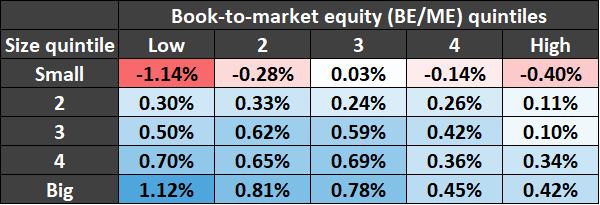
\includegraphics[width=0.55\linewidth]{A4.png}
	\label{fig:label}
\end{figure}

\section{Time-series Regression Results}


After performing linear regression for 25 portfolios between 2011-2018, coefficients for all regressors have been summarized in Table 5. First of all, for intercept a, we are unable to reject null hypothesis in 24/25 portfolios, except for the portfolio on the upper left corner as highlighted. This is to convey there is no abnormal return in FF-3 factor model, which implies its capability in explaining stock return variation. Secondly, t-test results for slope b suggest rejection of null hypothesis. As anticipated, values of slope b are close to 1. Thirdly, t-statistics are strong enough to reject null hypothesis for s (slope for SMB) in four smaller size quintiles. The exception happens for “Big” size quintiles where slopes turn negative as highlighted. Similarly, for HML, t-tests are not able to reject null hypothesis when h turns into positive from lower BE/ME quintile to higher BE/ME quintile.

\begin{figure}[h]
	\centering
	\caption*{Table 5: Regression Summary for FF3 Model 2011-2018}
	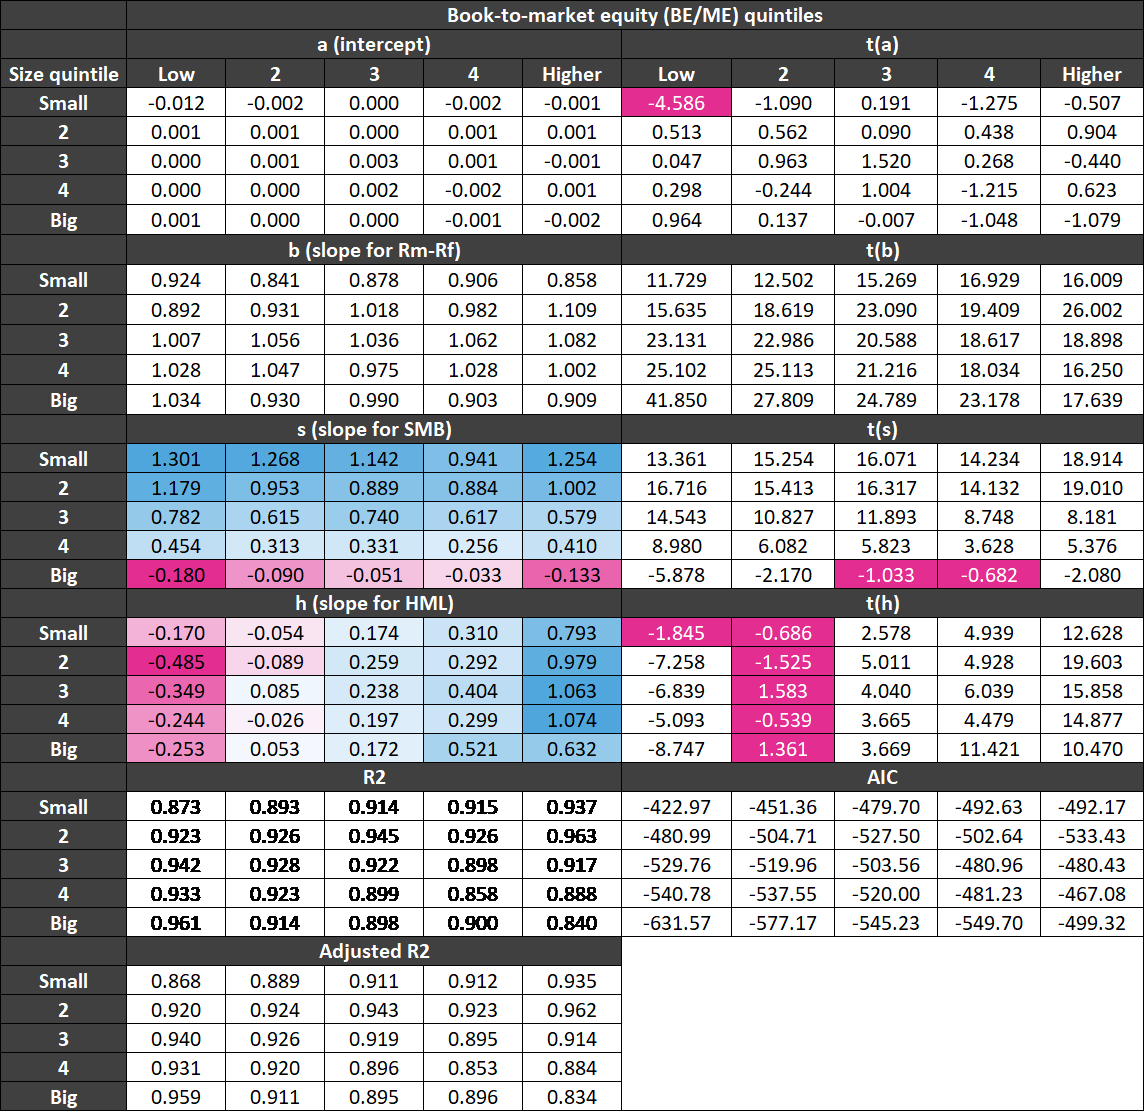
\includegraphics[width=1\linewidth]{A5.png}
	\label{fig:label}
\end{figure}


\noindent In order to prove stronger explanatory power of FF 3-factor model, regression analysis has also been conducted on single factor CAPM. Results are tabulated below. Generally, t-statistics for intercept are much higher than they are in FF 3 in absolute term. This implies abnormal returns vanish with introduction of SMB and HML. On the other hand, b values for CAPM tend to be higher than when they are in FF 3. Last but not least, discrepancies of R2 in Table 5 and Table 6 indicates FF 3-factor model improves the explanatory power from 50\%-90\% range (CAPM) to 84\%-96\% range. Adjusted R2 results double confirm the additional explanatory power that SMB and HML bring to the model. FF 3-factor models have lower AIC in all 25 portfolios than CAPM, suggesting its explanatory power comes without overfitting.



\begin{figure}[h]
	\centering
	\caption*{Table 6: Regression Summary for CAPM 2011-2018}
	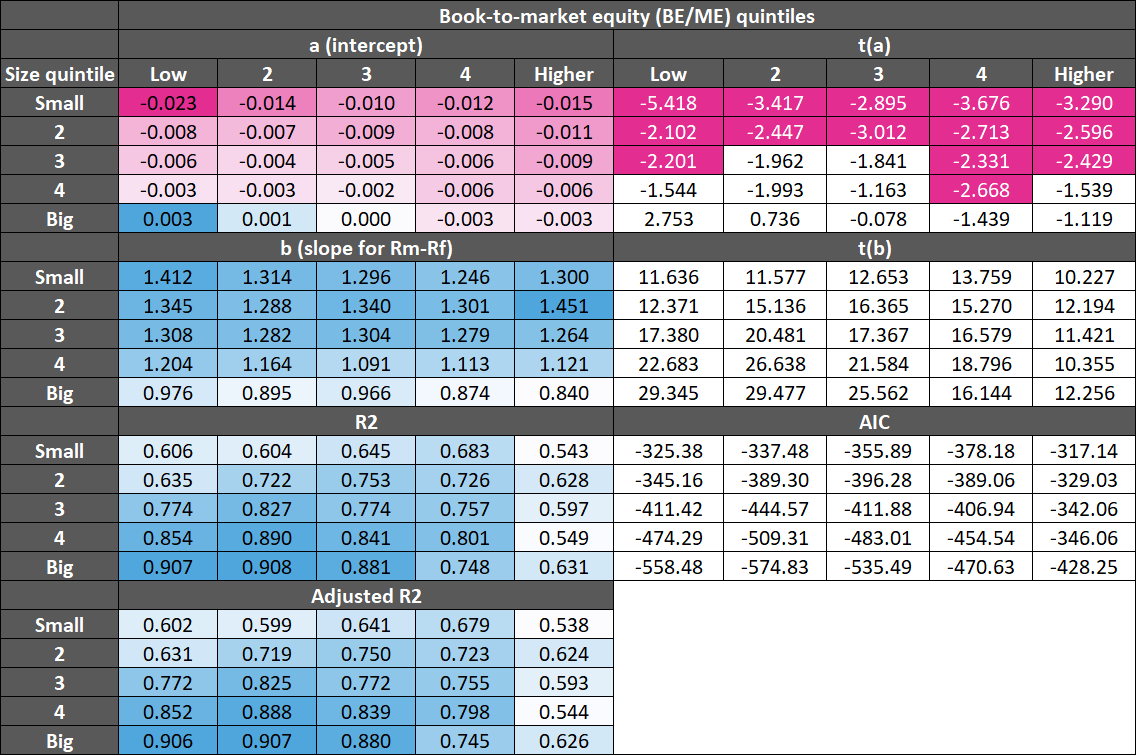
\includegraphics[width=1\linewidth]{A6.png}
	\label{fig:label}
\end{figure}

\section{Interpretation}

Fama and French explained size and BE/ME are not ad hoc variables for explaining average stock return(1992b). They believed both variables are related to economic fundamentals. Firms that have high BE/ME ratio tend to have low earnings on assets. The intuition is that investors would not be attracted by firms that have poor earning performance recently. Reversely, investors tend to invest in firms with strong earning/profitability figure recently (1992b). Size is also related to profitability. Fama and French attributed size effect to smalls firms not able to participate in economic boom of the middle and late 1980s, which pushed small firms to a long earnings depression. However, their paper in 1992b and 1993 did not explain how size and BE/ME’s relationship with earning leads to their relationship with average excess returns (of 25 portfolios).

\noindent Practitioners have been debating on whether the outperformance tendency is due to market efficiency or inefficiency. The “inefficiency” proponents believe the outperformance is explained by incorrectly value pricing of companies by market participants. However, the “inefficiency” rhetoric does not explain why small firms were mispriced higher instead of lower.

\noindent Market efficiency seems to explain this more logically. Intuition comes as: in old days such as 1963-1991, it was not easy for investors to access to or liquidate small-cap stocks. In addition, small firms normally have higher cost of capital and greater business risk. All of these made small-cap stocks riskier to invest, hence higher return in old days. On the other hand, it is much easier for investors to access to small-cap stocks and liquidate nowadays. More transparent market also reduces risk of investing in small firms. These could explain why small cap stocks does not outperform large cap stocks as they used to be.

\noindent We are still able to see News nowadays saying samll cap's outperformance tendency exists. This is not true for US equities tested between 2011-2018 in this paper. Flaw of these News was their neglect of "Survivorship Bias". According to Elton, Gruber, and Blake (1996), survivorship bias is larger in the small-fund sector than in large mutual funds. Small caps are easier to go bankrupcy and being excluded from analysis. 


	\section{Conclusion} % Numbered section
	\noindent In conclusion, we have accomplished our research objective to prove that Fama and French three-factors model does significantly explain the returns of stocks listed on the NYSE, NASDAQ and AMEX for the period between Jul 2011 – Dec 2018. Together with the observed market data and collected statistical significance results, all quintiles, except for certain Big-Sized portfolios and Low Book-to-Market quintiles, produce high t-stat values results which means the coefficients are statistically significant, and this is coherent to Fama and French (1993).  Beyond beta, Fama and French found that small-sized companies often gained higher returns than those of larger-sized companies, while value stocks (Low Book-to-Market equity) gained higher returns than those associated with growth stocks (High Book-to-Market equity). The intuition is that higher compensation is necessary for riskier investments, which results in higher earnings potential. Another intuition is that smaller companies attract less attention and are more likely to be mispriced.\\
	
	\noindent Evident in the Fama and French (1996) paper, the intercepts are strongly negative for short-term-losers and strongly positive for short-term winners for the observed period from t-2 to t-12 months. This therefore highlights the fact that the original three-factor model fails to capture the short-term momentum anomalies, in which set forth Cahart’s research in incorporating momentum into the original Fama and French three-factor model. Lately, research has also further spurred the development of other risk factors, such as liquidity, investment, and profitability factors (Pastor and Stambaugh,
	2003; Fama and French, 2015; Hou, Xue, and Zhang, 2015), to be incorporated into the model to further improve the explanatory power of the models and formulate trading strategies; However, factor models might vary in different markets, and one therefore has to be prudent in the same factor model application across different markets. \\


	\section{References} % Numbered section
	\begin{itemize}
		\item Markowitz, H. (1952). Portfolio selection. The Journal of Finance, 7(1), 77-91.
		\item Sharpe, W. (1964). Capital asset prices: A theory of market equilibrium under conditions of risk. Journal of Finance, 19(3), 425-442.
		\item Lintner, J. (1965). The valuation of risk assets and the selection of risky investments in stock portfolios and capital budgets. Review of Economics and Statistics, 47(1), 12-37.
		\item Fama, E., \& French, K. (1993). Common risk factors in the returns on stocks and bonds.Journal of Financial Economics, 33(1), 3-56..
		\item Black, Fischer. Michael C. Jensen. and Myron Scholes. 1971. The capital asset pricing model: Some empirical tests. in: M. Jensen. ed.. Studies In the theory of capital markets (Praeger, New York, NY).
		\item Fama. Eugene F. and Kenneth R. French. 1992a. The cross-section of expected stock returns.Journal of Finance 47, 427 - 465.
		\item Fama. Eugene F. and Kenneth R. French. 1992b. The economic fundamentals of size and book-to-market equity. Working paper (Graduate School of Business. Cniversity of Chicago. Chicago. IL).
		\item Elton; Gruber; Blake (1996). "Survivorship Bias and Mutual Fund Performance"
		\item Banz. Rolf W.. 1981. The relationship between return and market value of common stocks, Journal	of Financial Economics 9. 3-15.
		\item Bhandari. Laxmi Chand. 1983. Debt,equity ratto and e.xpected common stock returns: Empirical evidence, Journal of Finance 43. 507-528.
		\item Rosenberg. Barr, Kenneth Reid. and Ronald Lanstein. 1985. Persuasive evidence of market inefficiency.Journal of Portfolio Management Il. 9-17.
		\item Stattman D (1980): Book values and stock returns. The Chicago MBA: A Journal of Selected Papers,4,25–45. 
		\item Basu. Sanjoy. 1983. The relationship between earnings yield. market value. and return for NYSE common stocks: Further evidence. Journal of Financial Economics 12, 129-156.
		\item Daniel, K., \& Titman, S. (1997). Evidence on the characteristics of cross sectional variation in stock returns
		\item Davis, J., Fama, E.,\& French, K. (2000). Characteristics, covariances and average returns: 1927-97. Journal of Finance, 55(1), 389-406
		\item Fama. Eugene F. and Kenneth R. French. 1996. Multifactor Explanations of Asset Pricing Anomalies. Journal of Finance, 51(1), 55--84
		\item Pastor, L., Stambaugh, R.F., 2003. Liquidity risk and expected stock returns. Journal of Political Economy 111, 642–685.
		\item A five-factor asset pricing model. Journal of Financial Economics 116, 1–22.
		\item Hou, K., Xue, C., Zhang, L., 2015. Digesting anomalies: An investment approach. Review of Financial Studies 28, 650–705.
	\end{itemize}


\end{document}
© 2019 GitHub, Inc.
Terms
Privacy
Security
Status
Help
Contact GitHub
Pricing
API
Training
Blog
About
